\chapter{Implementation}

The implementation of OpenArmor follows a phased approach, integrating advanced logging techniques, AI-driven analysis, and established security tools. Each phase builds upon the previous, creating a comprehensive and intelligent cybersecurity solution.

\section{Phase 1: Advanced Logging and Data Collection}

\subsection{eBPF Logging Implementation}
\begin{itemize}
    \item Develop custom eBPF programs for efficient kernel-level event capture
    \item Implement a user-space daemon to collect and buffer eBPF events
    \item Optimize eBPF programs for minimal system overhead
    \item Create interfaces for dynamically loading and unloading eBPF programs
\end{itemize}

\subsection{Integration of Existing Security Tools}
\begin{itemize}
    \item Deploy and configure Wazuh agents for host-based intrusion detection
    \item Implement OSquery for on-demand and scheduled system state queries
    \item Set up Sysmon for detailed Windows event logging
    \item Develop adapters for each tool to feed data into OpenArmor's central system
\end{itemize}

\subsection{Network Traffic Analysis}
\begin{itemize}
    \item Implement packet capture using libpcap or similar libraries
    \item Develop modules for protocol analysis and flow record generation
    \item Set up NetFlow/IPFIX collectors for network flow monitoring
\end{itemize}

\section{Phase 2: Log Standardization and Integration}

\subsection{OCSF Standardization Implementation}
\begin{itemize}
    \item Develop parsers for eBPF, Wazuh, OSquery, and Sysmon data formats
    \item Implement OCSF schema mapping and validation logic
    \item Create a flexible framework for adding new data source adapters
    \item Set up a centralized log storage system (e.g., Elasticsearch)
\end{itemize}

\subsection{Data Enrichment Pipeline}
\begin{itemize}
    \item Integrate geolocation databases for IP address enrichment
    \item Implement connectors for threat intelligence feeds
    \item Develop an asset management integration for system context
    \item Create a modular enrichment pipeline for easy extension
\end{itemize}

\section{Phase 3: AI Log Processing}

\subsection{Data Preprocessing}
\begin{itemize}
    \item Implement feature extraction and selection algorithms
    \item Develop modules for handling missing data and outliers
    \item Create data normalization and scaling pipelines
\end{itemize}

\subsection{Machine Learning Model Development}
\begin{itemize}
    \item Implement unsupervised learning models:
    \begin{itemize}
        \item Isolation Forest for outlier detection
        \item DBSCAN for density-based clustering
    \end{itemize}
    \item Develop supervised learning models:
    \begin{itemize}
        \item Random Forest for multi-class threat categorization
        \item Gradient Boosting for binary classification
    \end{itemize}
    \item Implement deep learning models:
    \begin{itemize}
        \item LSTM networks for sequence-based anomaly detection
        \item Autoencoders for dimensionality reduction
    \end{itemize}
\end{itemize}

\subsection{Natural Language Processing}
\begin{itemize}
    \item Implement text preprocessing for log messages
    \item Develop word embedding models for log semantics
    \item Create named entity recognition for identifying key elements in logs
\end{itemize}

\section{Phase 4: Automated Threat Detection}

\subsection{Rule-Based Detection Engine}
\begin{itemize}
    \item Implement a flexible rule engine supporting complex conditions
    \item Develop an interface for easy rule creation and management
    \item Integrate Wazuh's existing rule set into OpenArmor's engine
\end{itemize}

\subsection{Anomaly Detection System}
\begin{itemize}
    \item Implement statistical anomaly detection models
    \item Develop baseline profiling for normal system behavior
    \item Create adaptive thresholding for dynamic environments
\end{itemize}

\subsection{Behavior Analytics}
\begin{itemize}
    \item Implement user and entity behavior analytics (UEBA) models
    \item Develop graph-based analysis for entity relationship mapping
    \item Create behavior-based detection for advanced persistent threats
\end{itemize}

\subsection{Threat Intelligence Integration}
\begin{itemize}
    \item Implement connectors for major threat intelligence platforms
    \item Develop a local cache for efficient IoC lookups
    \item Create a feedback mechanism to contribute to threat intelligence
\end{itemize}

\section{Phase 5: Monitoring and Response}

\subsection{Real-Time Analytics Implementation}
\begin{itemize}
    \item Set up Apache Kafka for high-throughput event streaming
    \item Implement Apache Flink jobs for real-time data processing
    \item Develop custom sliding window algorithms for time-series analysis
\end{itemize}

\subsection{Alert Management System}
\begin{itemize}
    \item Implement a risk scoring algorithm for alert prioritization
    \item Develop an alert correlation engine to identify related events
    \item Create an automated alert enrichment pipeline
\end{itemize}

\subsection{Response Automation}
\begin{itemize}
    \item Develop integrations with firewalls and EDR solutions for automated blocking
    \item Implement a playbook engine for orchestrating response actions
    \item Create an AI-assisted decision support system for complex incidents
\end{itemize}

\subsection{User Interface and Dashboards}
\begin{itemize}
    \item Develop a web-based user interface using modern frontend frameworks
    \item Implement real-time data visualization components
    \item Create role-based access control for different user types
    \item Develop customizable dashboards for various security metrics
\end{itemize}

\begin{figure}[h]
    \centering
    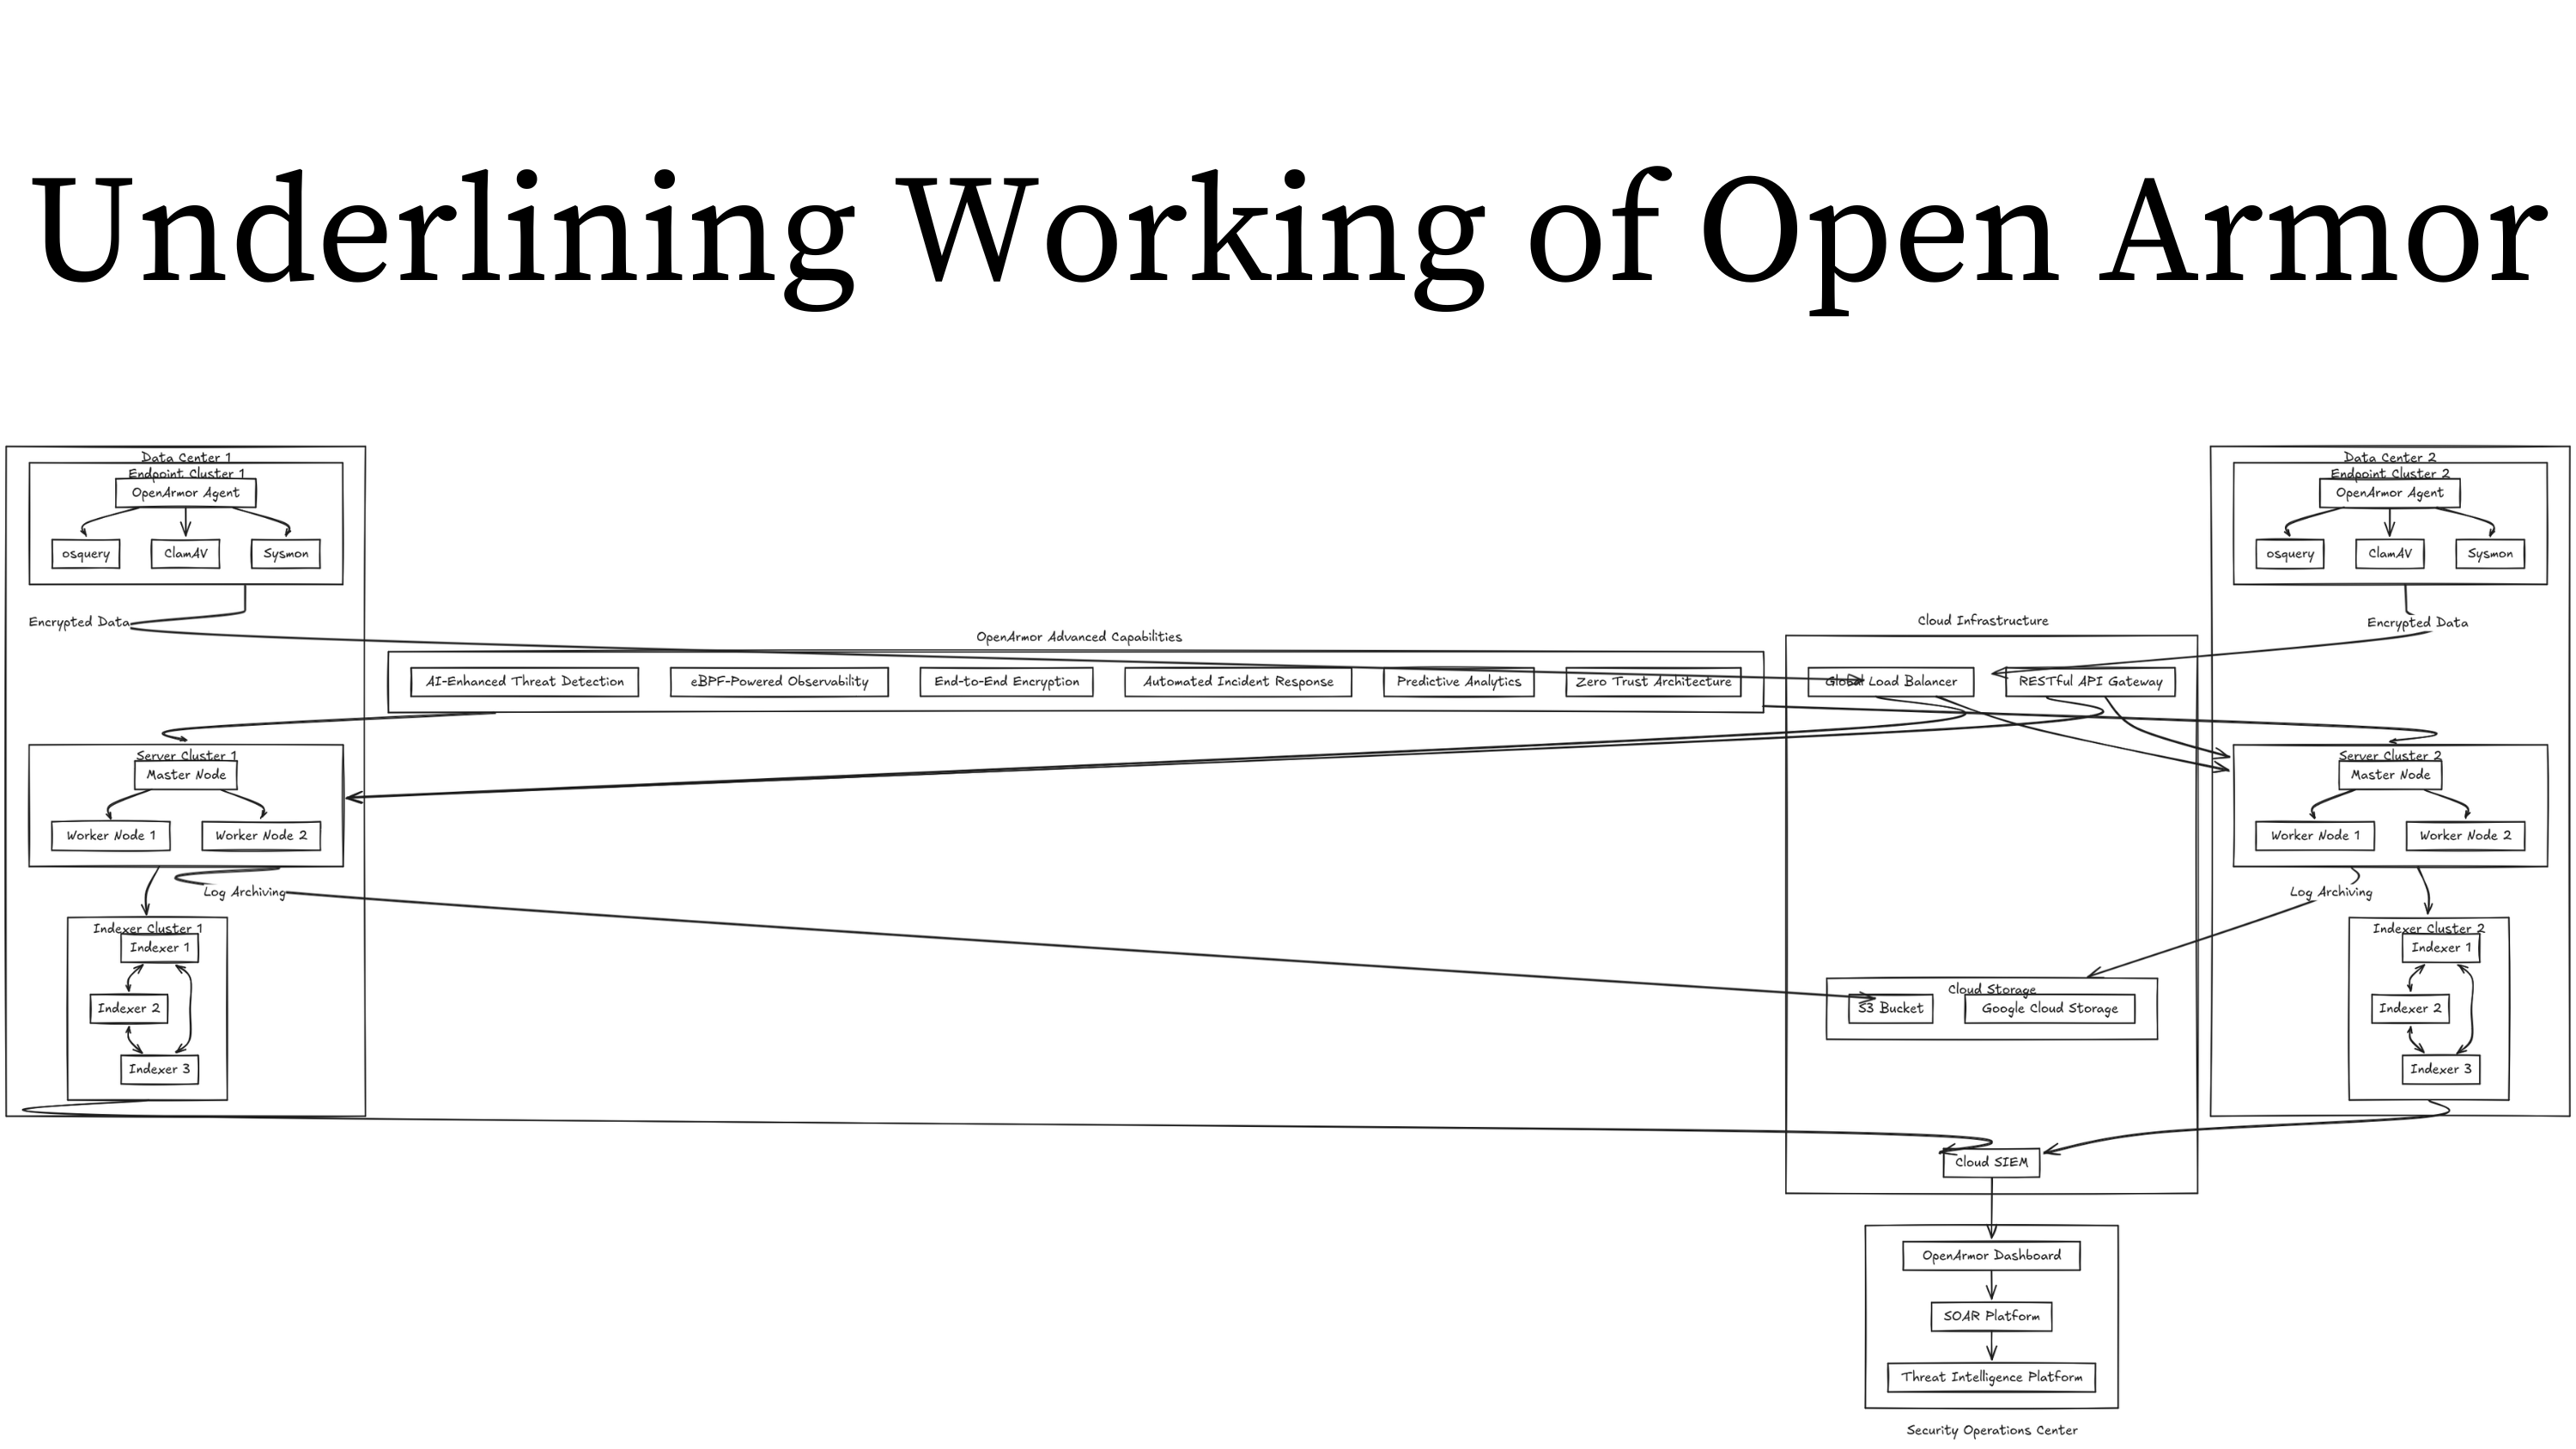
\includegraphics[width=1\linewidth]{working.png}
    \caption{OpenArmor Dashboard}
    \label{fig:openarmor-dashboard}
\end{figure}

\section{Phase 6: Continuous Improvement}

\subsection{Feedback Loop Implementation}
\begin{itemize}
    \item Develop interfaces for analysts to provide feedback on alerts
    \item Implement automated tracking of false positives and false negatives
    \item Create a system for continuous model performance evaluation
\end{itemize}

\subsection{Model Update Pipeline}
\begin{itemize}
    \item Implement automated model retraining schedules
    \item Develop A/B testing framework for new detection algorithms
    \item Create a versioning system for models and detection rules
\end{itemize}

\subsection{Threat Intelligence Gathering}
\begin{itemize}
    \item Implement a system for identifying and extracting new threat patterns
    \item Develop automated reporting of emerging threats
    \item Create a knowledge base for storing and retrieving threat information
\end{itemize}

\begin{figure}[h]
    \centering
    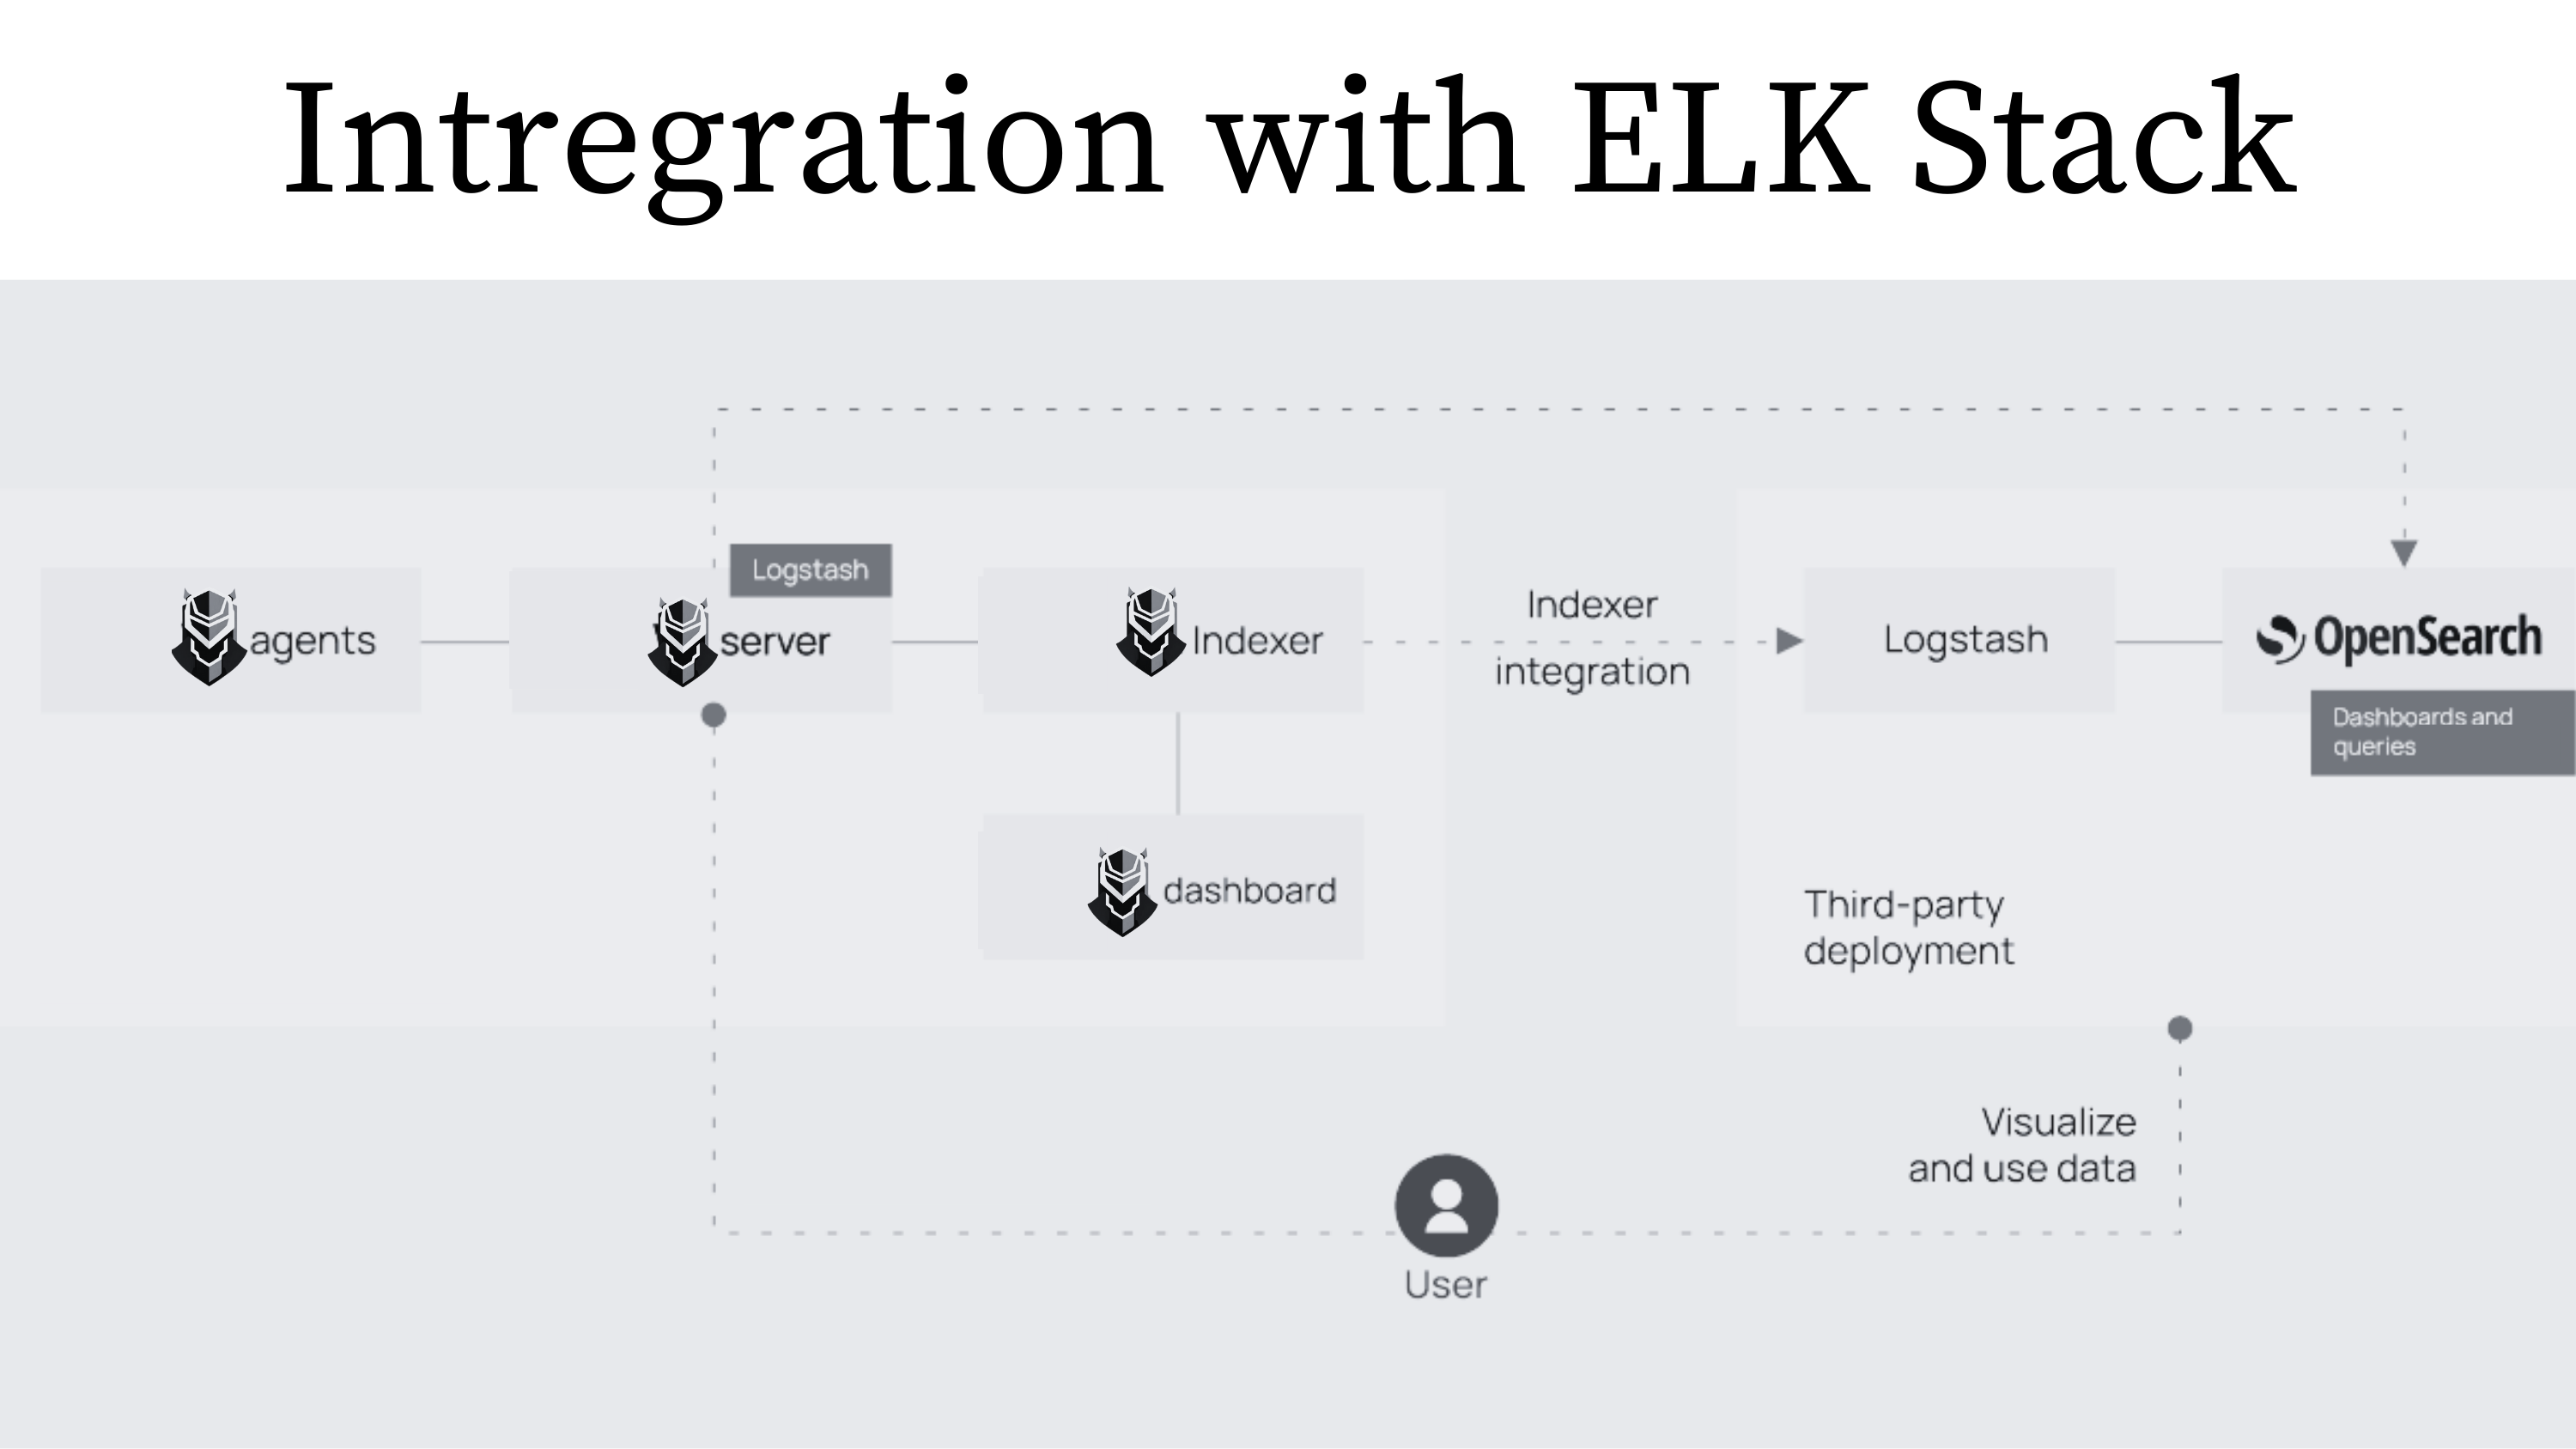
\includegraphics[width=1\linewidth]{integration-diagram-opensearch.png}
    \caption{OpenArmor Continuous Improvement Cycle for Amazon Opensearch and OpenSearch Dashboards}
    \label{fig:continuous-improvement-cycle}
\end{figure}

\section{Conclusion}

The phased implementation approach of OpenArmor ensures a systematic development of a comprehensive cybersecurity solution. By integrating advanced logging techniques, established security tools, and cutting-edge AI capabilities, OpenArmor provides a robust platform for threat detection, analysis, and response. The continuous improvement phase ensures that the system remains effective against evolving cyber threats, making OpenArmor a dynamic and adaptive security solution.